\documentclass[11pt]{article}


%opening

%%% PACKAGES
\usepackage[english]{babel}
\usepackage[T1]{fontenc} % pouzije EC fonty
\usepackage[utf8]{inputenc} % set input encoding (not needed with XeLaTeX) 
\usepackage{booktabs} % for much better looking tables
\usepackage{array} % for better arrays (eg matrices) in maths
\usepackage{paralist} % very flexible & customisable lists (eg. enumerate/itemize, etc.)
\usepackage{verbatim} % adds environment for commenting out blocks of text & for better verbatim

\usepackage{color}
\usepackage{xcolor}
\usepackage{listings}
\lstset{
	frame=top,frame=bottom,
	basicstyle=\small\normalfont\sffamily,    % the size of the fonts that are used for the code
	stepnumber=1,                           % the step between two line-numbers. If it is 1 each line will be numbered
	numbersep=10pt,                         % how far the line-numbers are from the code
	tabsize=2,                              % tab size in blank spaces
	extendedchars=true,                     %
	breaklines=true,                        % sets automatic line breaking
	captionpos=t,                           % sets the caption-position to top
	mathescape=true,
	stringstyle=\color{blue}\ttfamily, % Farbe der String
	keywordstyle=\color{blue}\ttfamily,
	commentstyle=\color{green}\ttfamily,
	showspaces=false,           % Leerzeichen anzeigen ?
	showtabs=false,             % Tabs anzeigen ?
	xleftmargin=17pt,
	framexleftmargin=17pt,
	framexrightmargin=17pt,
	framexbottommargin=5pt,
	framextopmargin=5pt,
	showstringspaces=false      % Leerzeichen in Strings anzeigen ?
}

\usepackage{caption}
\usepackage{subcaption}
%\usepackage[demo]{graphicx}

%\usepackage{pdfpages}


% Potřeba pro matematické vzorec a align
\usepackage{amsmath}
\usepackage{graphicx} % support the \includegraphics command and options
\usepackage{geometry}
\usepackage{float}
\usepackage{wrapfig}
\usepackage{cite}

\geometry{left=1in, right=1in}

\numberwithin{equation}{section}

\title{ROVI\\ Vision-Mini-Project 1}
\author{Petr Batek, Bjarki Páll Sigurðsson}


\begin{document}
\selectlanguage{english}

\maketitle

\newpage

\section{Image4\_1}

\begin{figure}[h]
	\vspace{-3cm}
	\centering
	\begin{subfigure}[b]{0.3\textwidth}
		\includegraphics[width=\textwidth]{fig/padded4_1.png}
		\caption{Padded}
		\label{fig:padded}
	\end{subfigure} \qquad
	 %add desired spacing between images, e. g. ~, \quad, \qquad, \hfill etc. 
	 %(or a blank line to force the subfigure onto a new line)
	\begin{subfigure}[b]{0.55\textwidth}
		\includegraphics[width=\textwidth]{fig/Image4_1.png}
		\caption{Original}
		\label{fig:image4_1}
	\end{subfigure}\qquad
	\caption{Image4\_1.png}
\end{figure}

It is possible to see a periodic defect in the image \ref{fig:image4_1}. After first view, the most evident defect are lines in diagonal direction. The information about the defect periodicity suggests to use frequency domain filtering, which is useful in removing periodic defects.
It is necessary to padd the image before Fourier transform computation in order to avoid wraparound error. Padded image is on Figure \ref{fig:padded}.

There is magnitude spectrum of Fourier transform of the image on the Figure \ref{fig:imgMagSpec}. One can notice peak values in each of the spectrum quadrants. Two peaks closer to the origin (center of spectrum) corresponds to diagonal lines, which are apparent in the image. However, there are two other peaks. They represent another parasitic frequency, which is not so apparent in the original image. To correct defects in the image without disturbance of other incorrupted features, selective filtering has to be used. Therefore Butterworth notch filter was designed according to expression (4.10-5) in the course book \cite{gonzwoods}.  

We found four parasitic frequency peaks in the magnitude spectrum. When designing a filter, it is important to get coordinate indexes of the peaks with respect to the center of the magnitude spectrum. This is the centre of spectrum coordinate frame. For transformation of pixel indexes, we thus computed the half of each picture dimension.
\begin{equation*}
	\left[O_{spectr}\right]^{image} =
	\begin{bmatrix}
	 u & v \\
	\end{bmatrix}^{image}
	= 
	\begin{bmatrix}
	1536 & 2400 \\
	\end{bmatrix}
\end{equation*}
Coordinates of four high intensity pixels were:
\begin{align*}
	\left[p_{1}\right]^{spectr} &= 
	\begin{bmatrix}
	u_1 & v_1 \\
	\end{bmatrix}^{spectr}
	= 
	\begin{bmatrix}
	u_1 & v_1 \\
	\end{bmatrix}^{image} - \left[O_{spectr}\right]^{image} \\
	&= \begin{bmatrix}
	2143 & 1771 \\
	\end{bmatrix}^{image}
	-
	\begin{bmatrix}
	1536 & 2400 \\
	\end{bmatrix}
	= 
	\begin{bmatrix}
	607 & -629 \\
	\end{bmatrix}
	\\
	\left[p_{-1}\right]^{spectr} &= 
	\begin{bmatrix}
	-607 & 629 \\
	\end{bmatrix}
	\\
	\left[p_{2}\right]^{spectr} &= 
	\begin{bmatrix}
	-203 & -200 \\
	\end{bmatrix}
	\\
	\left[p_{-2}\right]^{spectr} &= 
	\begin{bmatrix}
	203 & 200 \\
	\end{bmatrix}
\end{align*}
Computed values were used in the equation (4.10-5) as values of $\left[u_k\; v_k\right]$. The magnitude spectrum of a single notch filter is symmetrical with respect to beginning of spectrum coordinate system. Because of this property our final notch filter was composed only from 2 basic notch filters (instead of 4). Magnitude spectrum of the input image, filter and resulted filtered spectrum are on Figure \ref{fig:magspecs410}.

\begin{figure}[h]
	\centering
	\begin{subfigure}[b]{0.3\textwidth}
		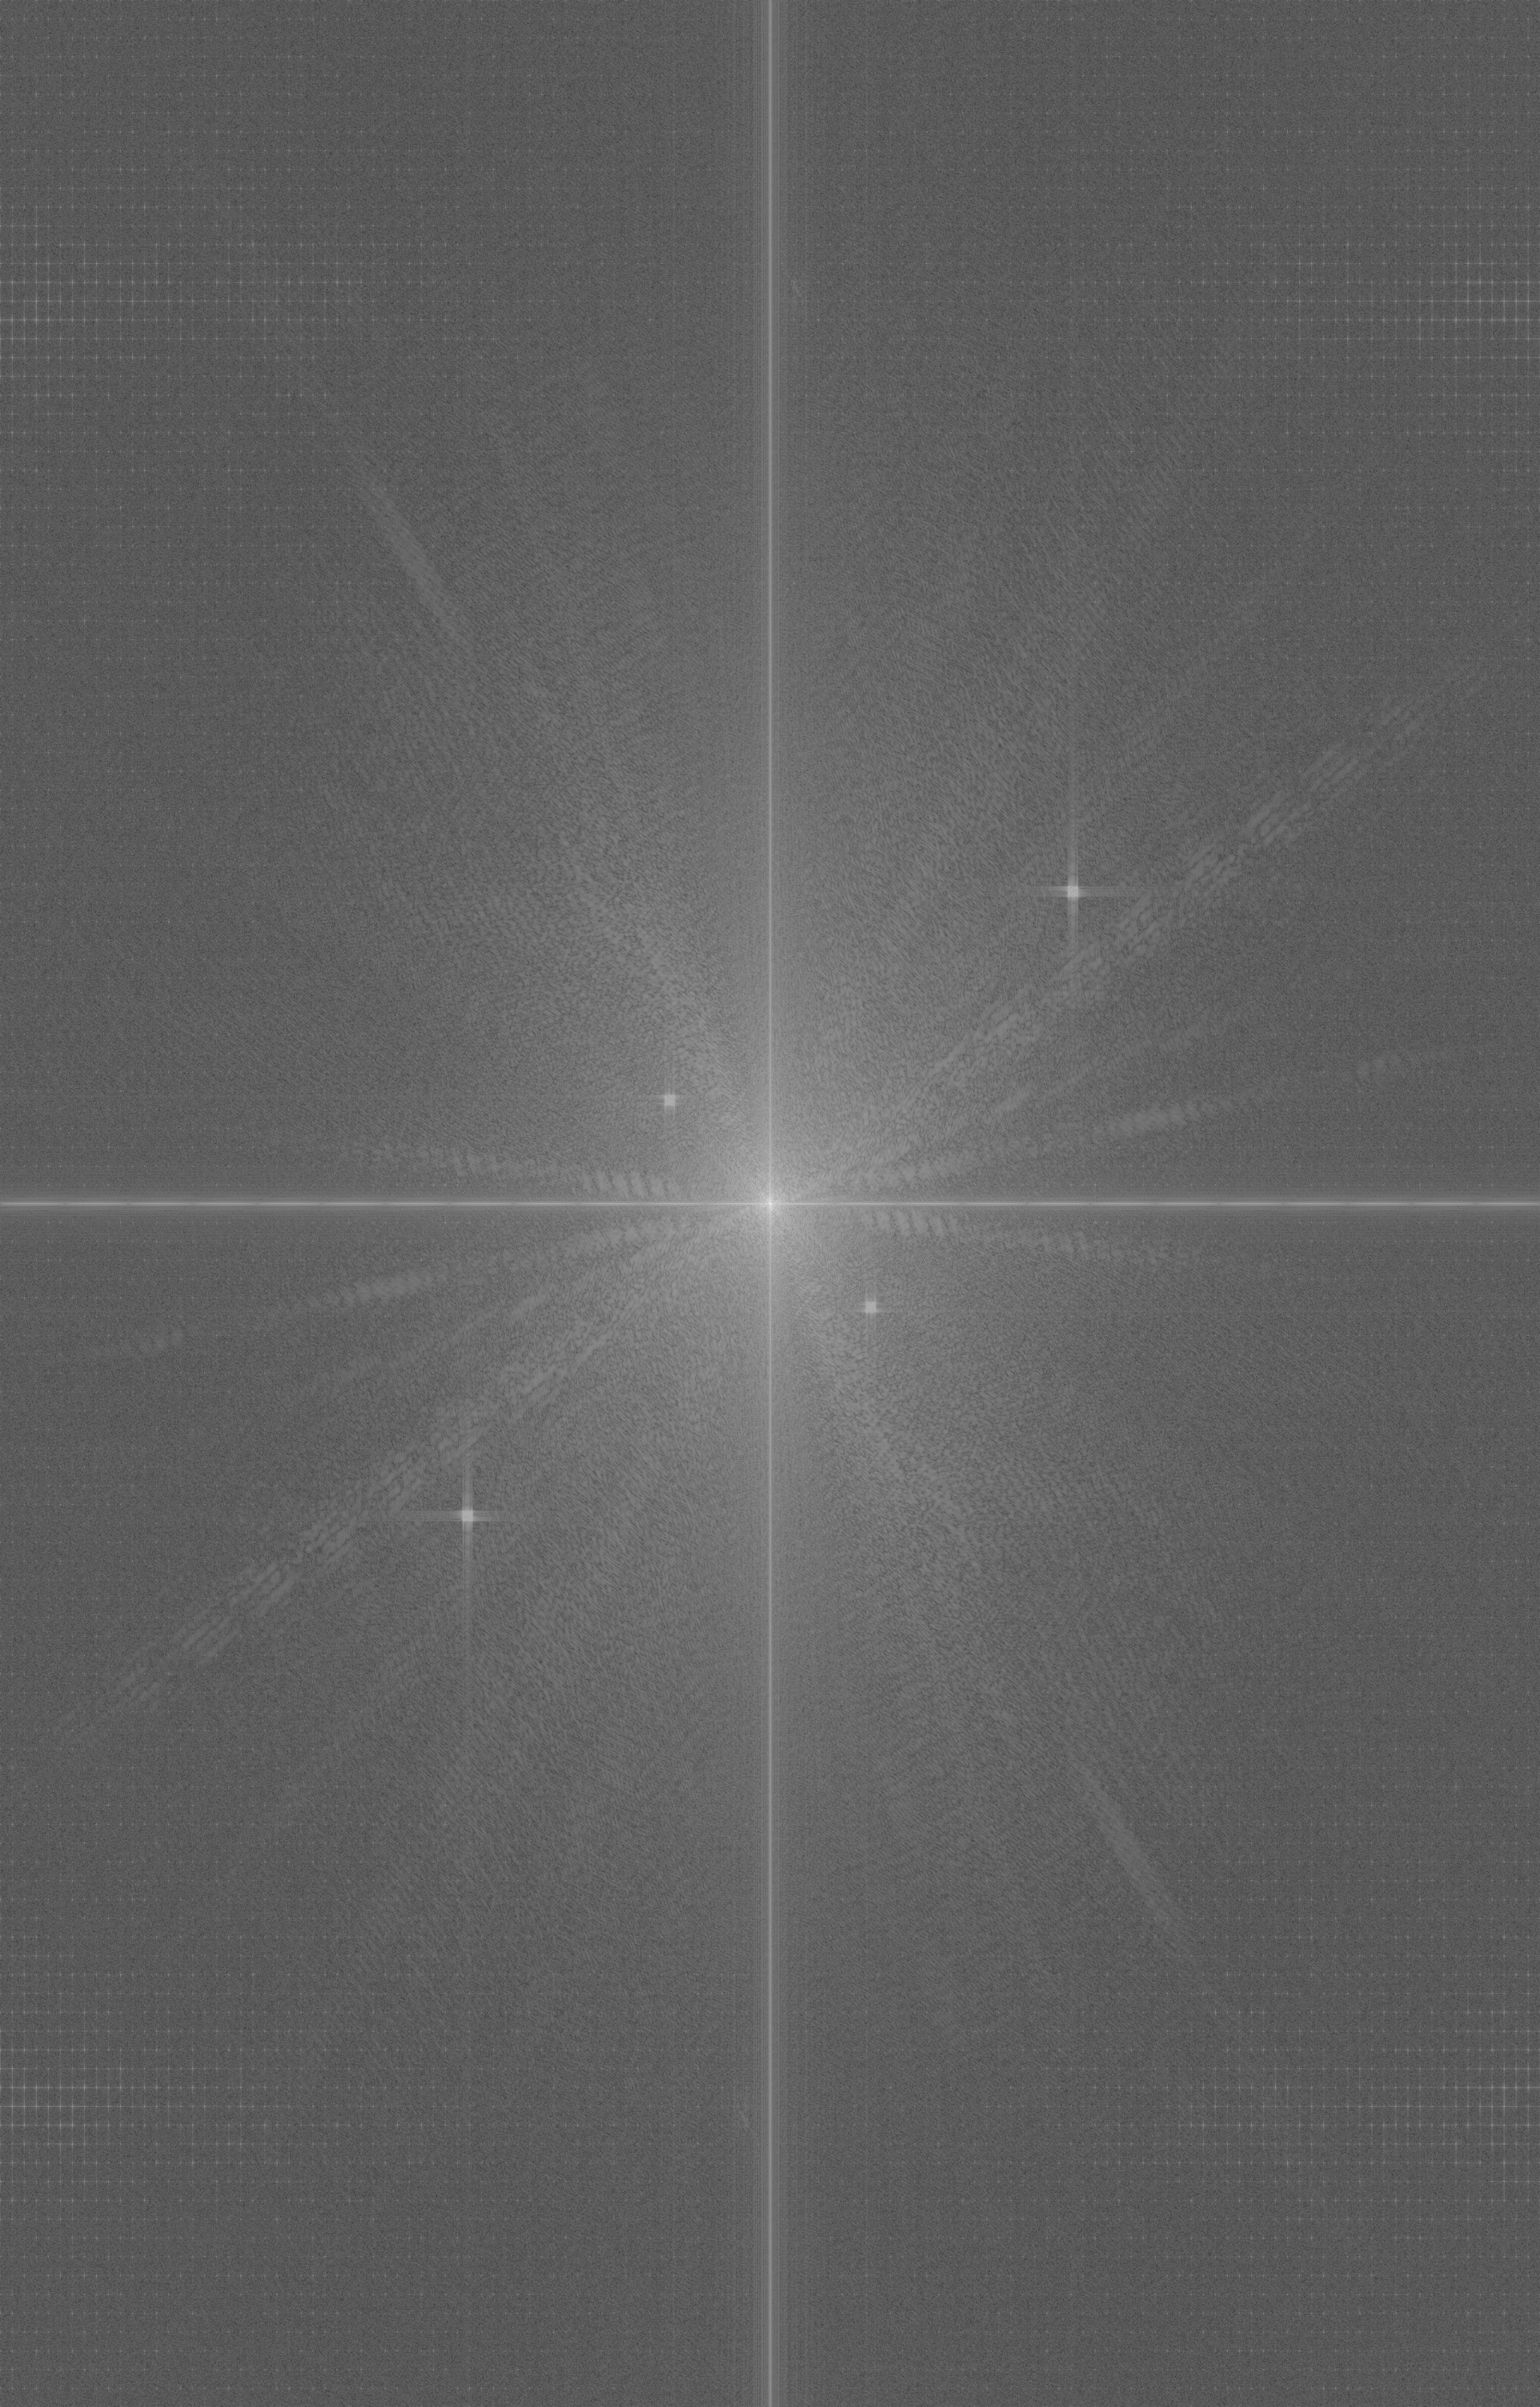
\includegraphics[width=\textwidth]{fig/mgSpec4_1.png}
		\caption{Mg. Spectrum of Image}
		\label{fig:imgMagSpec41}
	\end{subfigure} \quad
	\begin{subfigure}[b]{0.3\textwidth}
		\includegraphics[width=\textwidth]{fig/notchRF4_1.png}
		\caption{Butterworth Notch Filter}
		\label{fig:buttnotchfilter41}
	\end{subfigure}\quad
	\begin{subfigure}[b]{0.3\textwidth}
		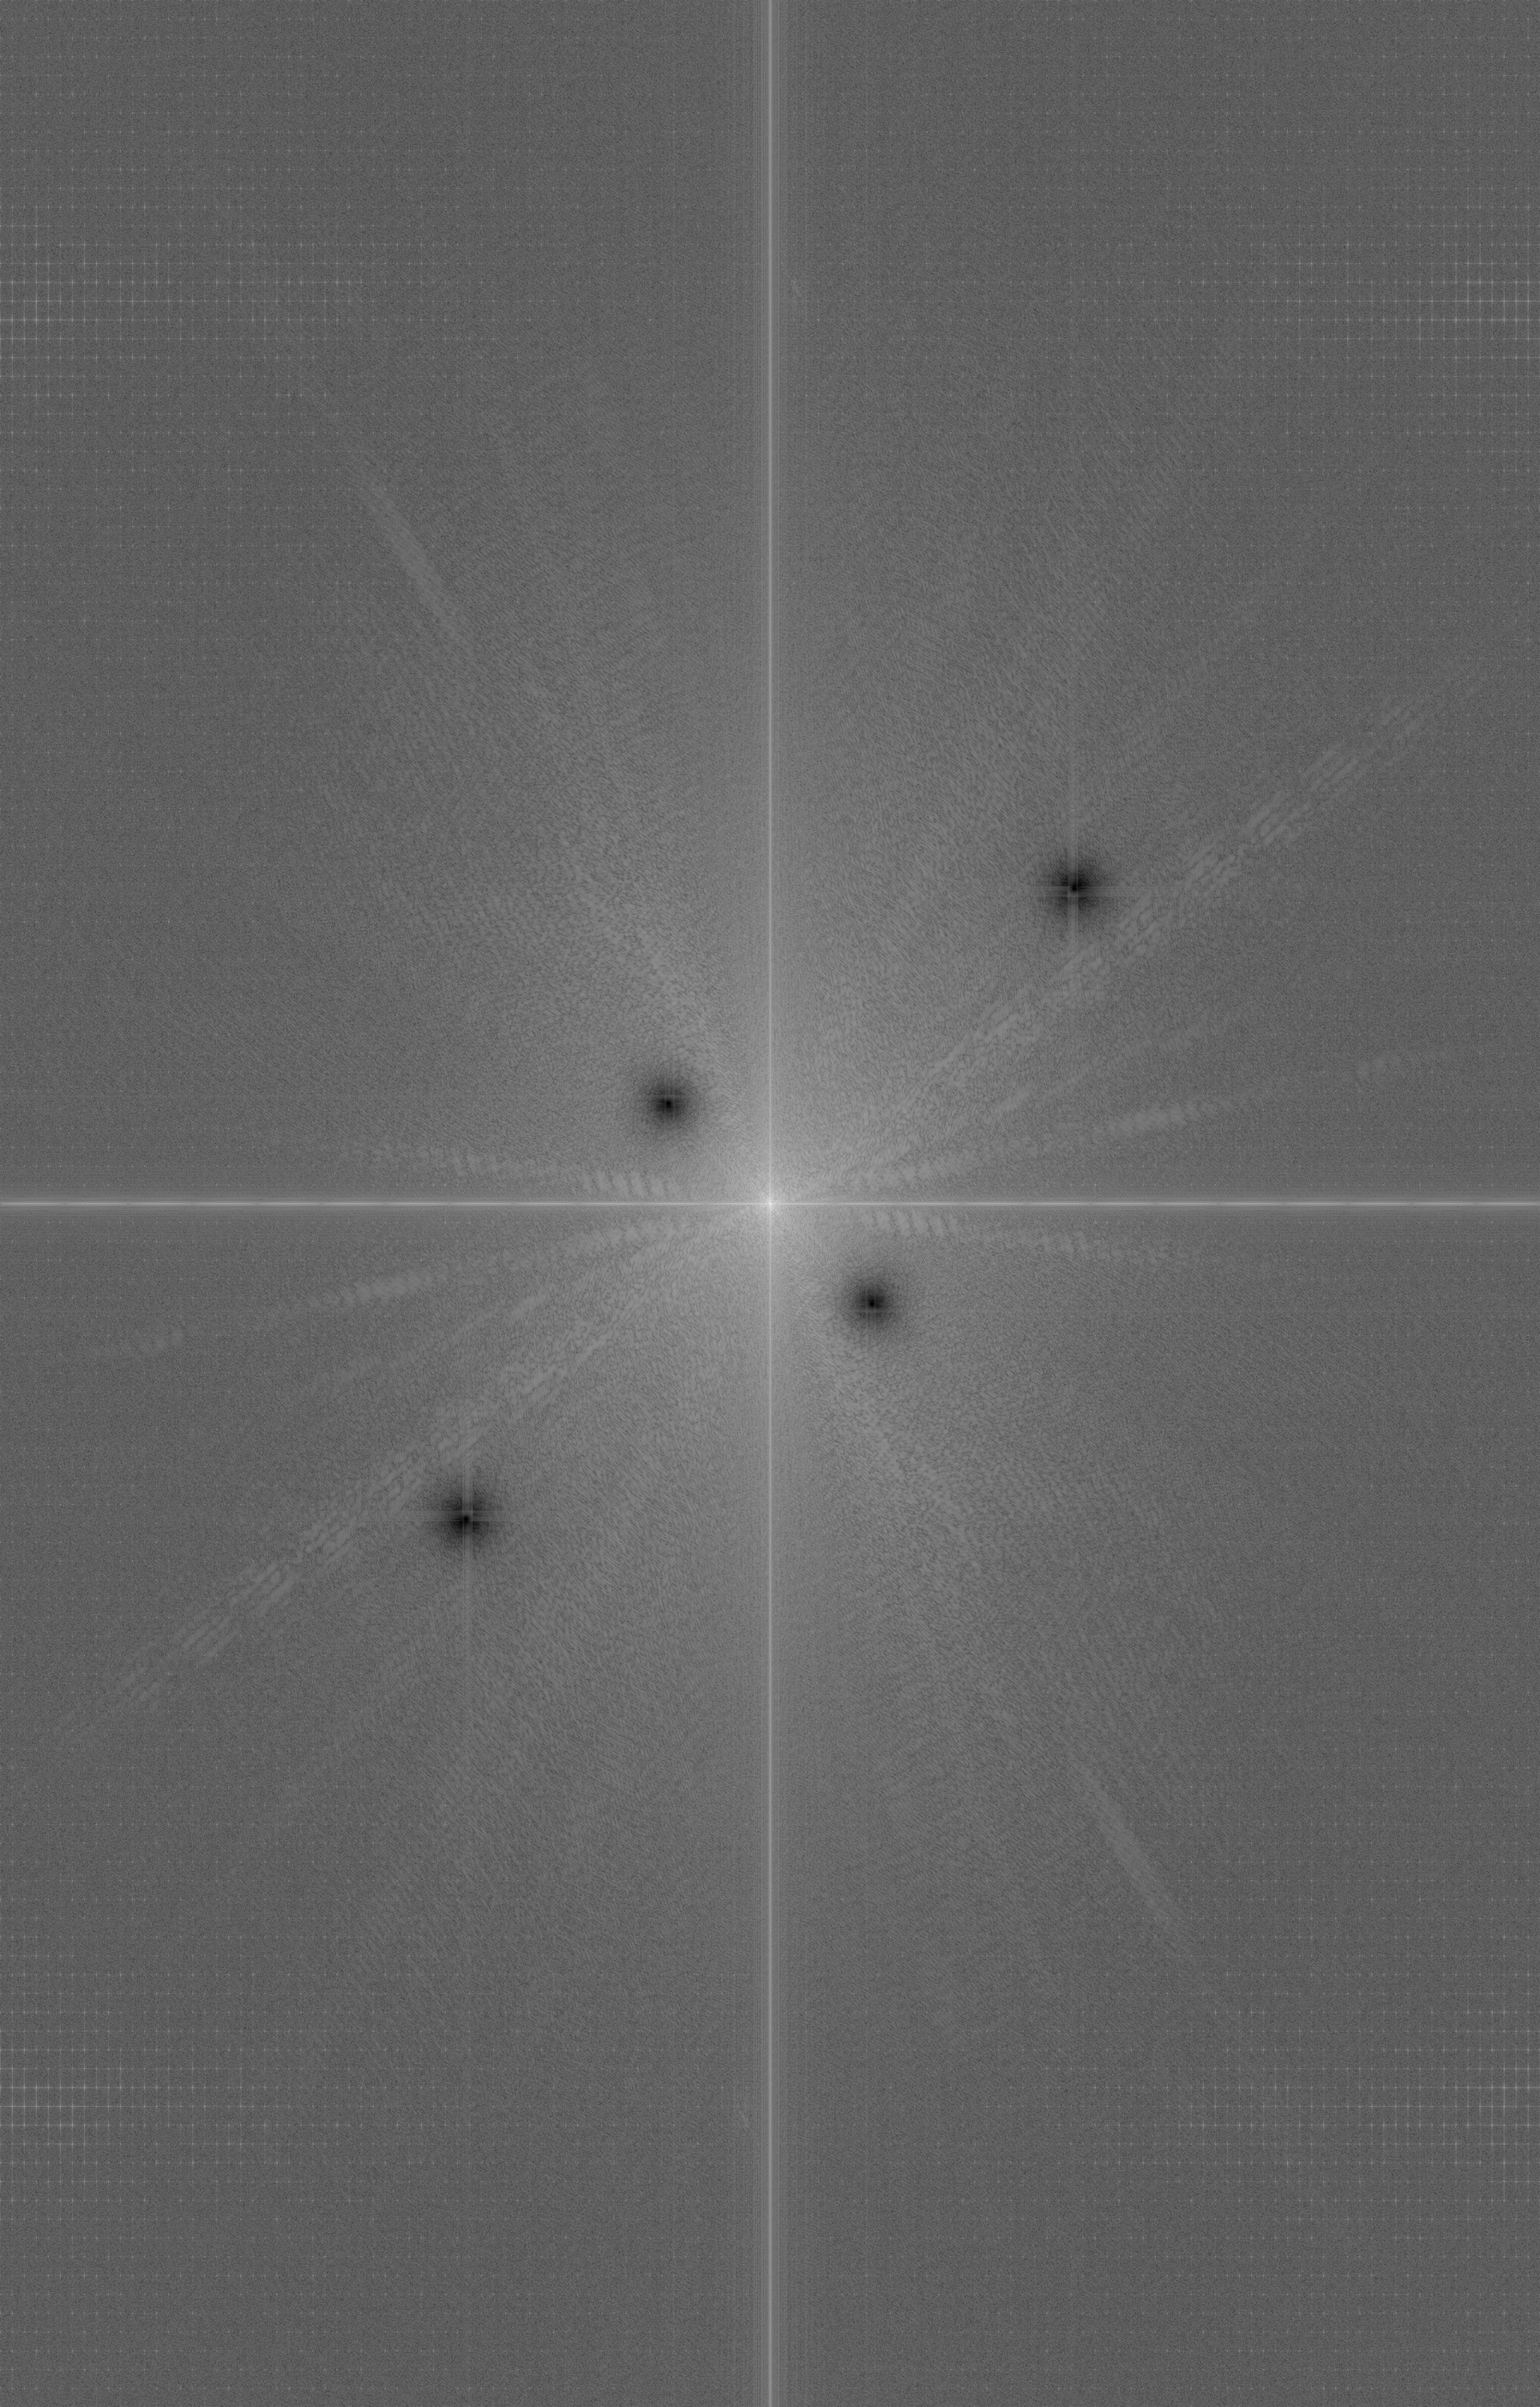
\includegraphics[width=\textwidth]{fig/FilteredSpectrum4_1.png}
		\caption{Filtered Mg. Spectrum}
		\label{fig:filteredMgSpectrum41}
	\end{subfigure}
	\caption{Frequency filtering}
	\label{fig:magspecs41}
\end{figure}

\begin{figure}[t]
	\centering
	\vspace{-2.5cm}
	\includegraphics[width=0.6\textwidth]{fig/OutputImage4_1.png}
	\caption{Filtered image}
	\label{fig:outputimage41}
\end{figure}

\newpage
You can see filtered output image on the Figure \ref{fig:outputimage41}. Improvement in the image quality is apparent and all parasitic lines in the image were cleared out.


\newpage
\section{Image4\_2}
\begin{figure}[h]
	\centering
	\begin{subfigure}[b]{0.4\textwidth}
		\includegraphics[width=\textwidth]{fig/Image4_2.png}
		\caption{Input Image}
		\label{fig:inputimage42}
	\end{subfigure} \qquad
	%add desired spacing between images, e. g. ~, \quad, \qquad, \hfill etc. 
	%(or a blank line to force the subfigure onto a new line)
	\begin{subfigure}[b]{0.4\textwidth}
		\includegraphics[width=\textwidth]{fig/OutputImage4_2.png}
		\caption{Filtered Image}
		\label{fig:outputimage42}
	\end{subfigure}\qquad
	\caption{Filtering of Image4\_2}
\end{figure}
There are also apparent periodic parasitic patterns in the Image4\_2 (fig. \ref{fig:inputimage42}). There would be also possible to apply a notch reject filter. However in this case, it would be necessary to compose final filter from 4 basic notch filters. Band stop filter is a better choice in this situation for this reason. Thus we designed a Butterworth band stop filter according to Table 4.6 from book \cite{gonzwoods}.

Spectrums of original image, designed filter and filtered image is depicted on Figure \ref{fig:magspecs42}.

Resulted filtered image is on the Figure \ref{fig:outputimage42}. Damaging periodic patterns are again gone.

\begin{figure}[h]
	\centering
	\begin{subfigure}[b]{0.3\textwidth}
		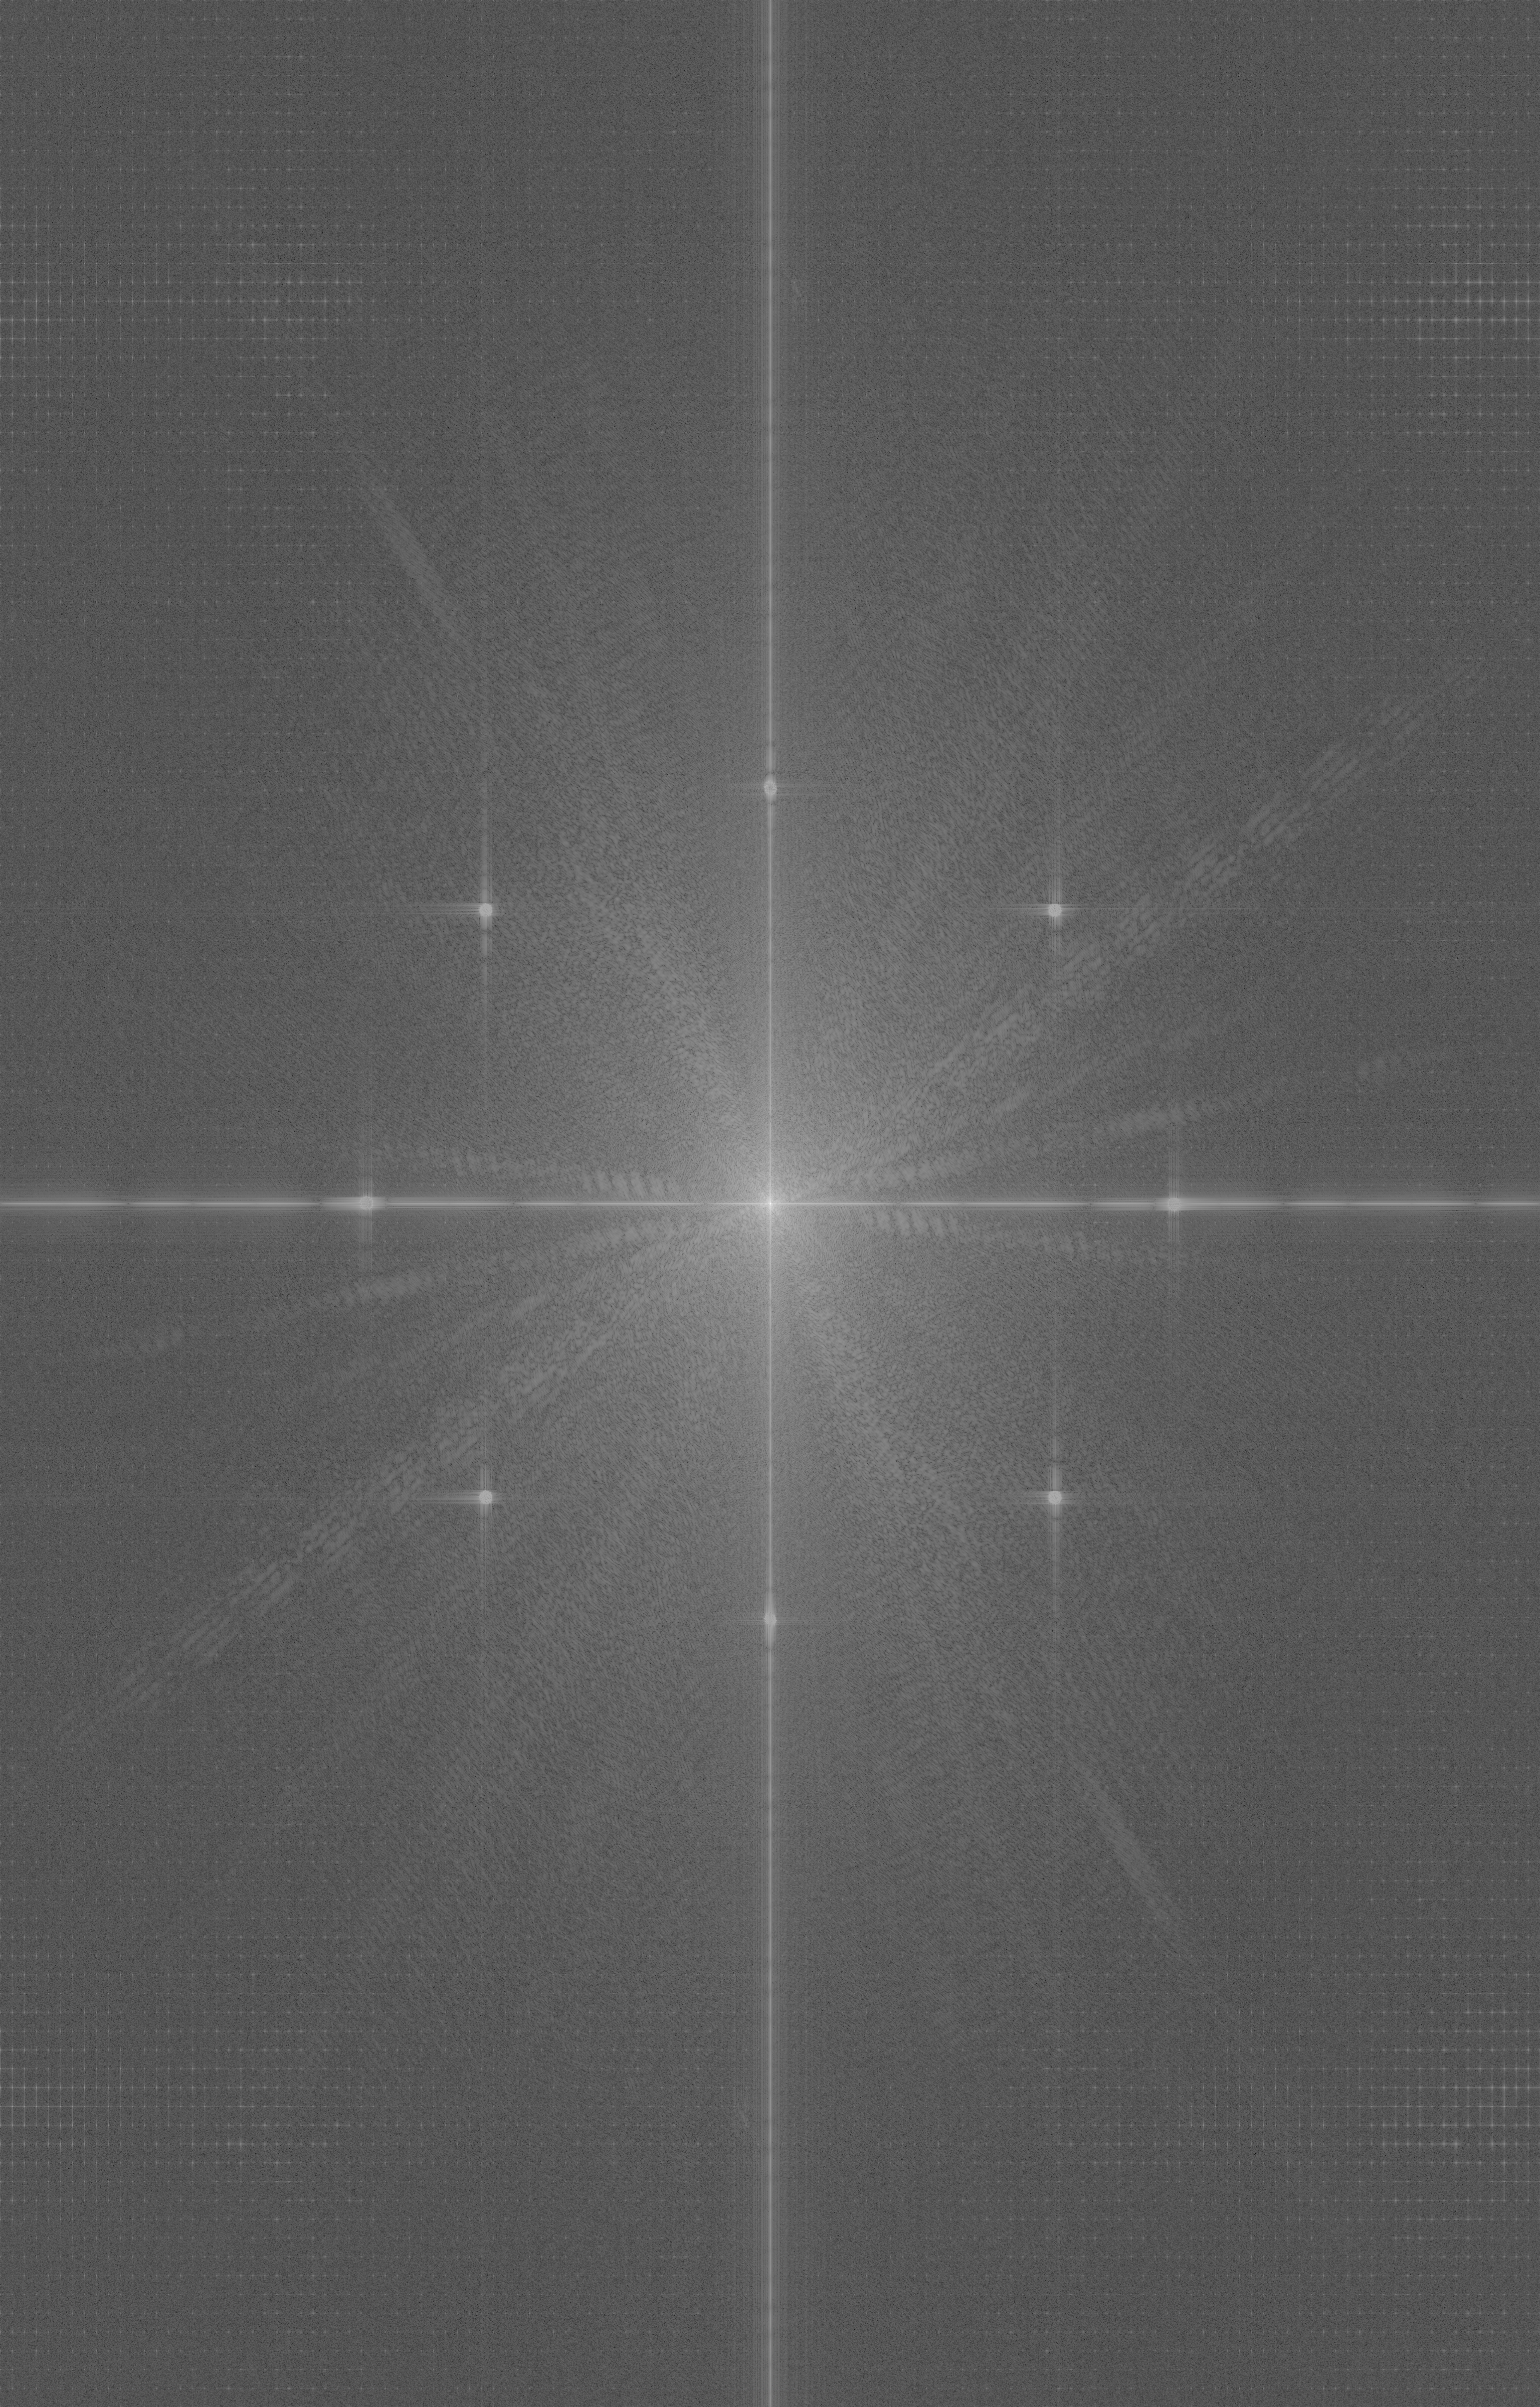
\includegraphics[width=\textwidth]{fig/mgSpec4_2.png}
		\caption{Mg. Spectrum of Image}
		\label{fig:imgMagSpec42}
	\end{subfigure} \quad
	\begin{subfigure}[b]{0.3\textwidth}
		\includegraphics[width=\textwidth]{fig/bandRF4_2.png}
		\caption{Butter. Band Stop Filter}
		\label{fig:buttnotchfilter42}
	\end{subfigure}\quad
	\begin{subfigure}[b]{0.3\textwidth}
		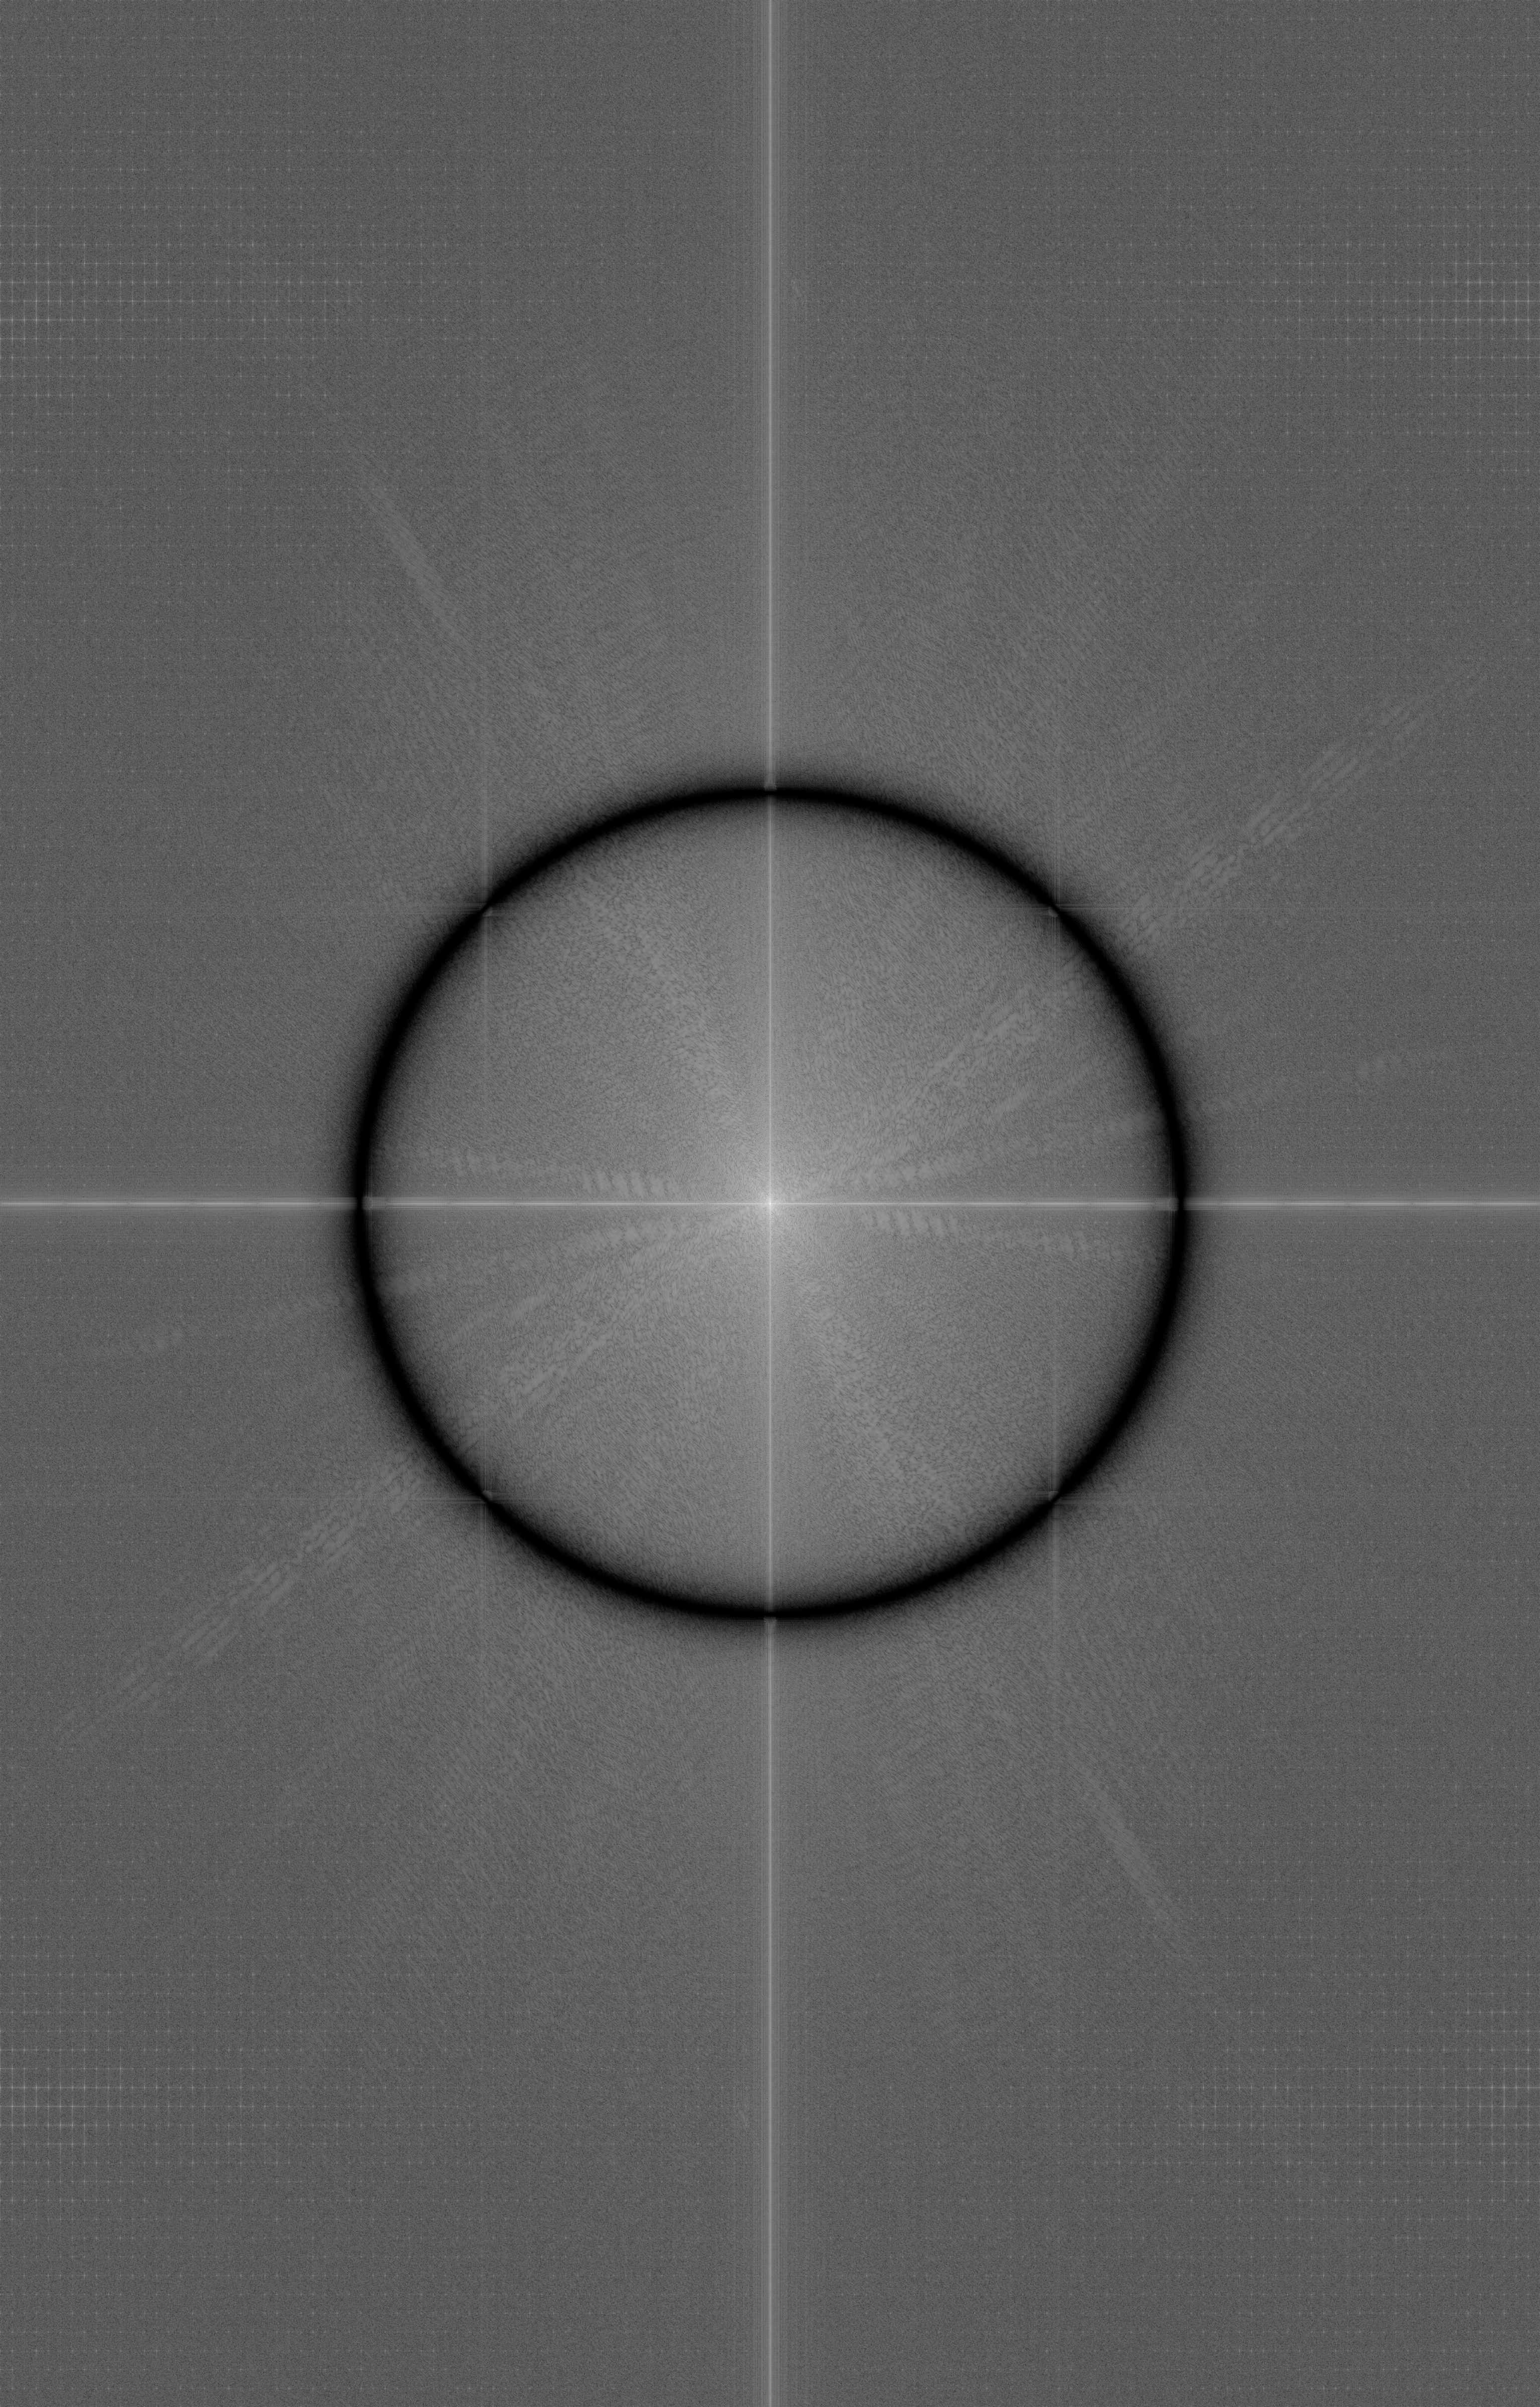
\includegraphics[width=\textwidth]{fig/FilteredSpectrum4_2.png}
		\caption{Filtered Mg. Spectrum}
		\label{fig:filteredMgSpectrum42}
	\end{subfigure}
	\caption{Frequency filtering}
	\label{fig:magspecs42}
\end{figure}

\newpage
\bibliographystyle{IEEEtran}
\bibliography{IEEEabrv,Sources}


\end{document}
